\section{Results}
\label{sec:Results}

\subsection{Requirements \& FL Solutions Comparison}
\label{subsec:ResultsRequirements}

% Reference to the table
\Cref{tab:ToolComparison} summarizes the results of our requirement analysis and the comparison of the FL solutions considered in this work. The identified requirements are described in more detail below. Please note that entries marked with a hyphen could not be determined with full confidence by the author team\footnote{Not all the available resources are detailed enough to allow a reliable classification.}.
The two entries marked by additional brackets are explained in \Cref{subsec:DiscussionRequirements}.

\begin{table}[htbp!]
\begin{adjustbox}{width=1\textwidth}
  \centering
  \begin{tabular}{llccccccc}
    \multicolumn{2}{c}{Requirement} & TFF & FedML & FATE & PaddleFL & PySyft & \makecell{NVIDIA Clara \\ Federated} & \makecell{JIP \\ Federated} \\
    \hline \\[-2.5ex] %[-1.5ex]
    
    \multicolumn{2}{l}{Open-source}                                             & \cmark & \cmark & \cmark & \cmark & \cmark & \xmark & \cmark \\
    \multicolumn{2}{l}{Offline installation}                                    & \xmark & \xmark & \xmark & \xmark & \xmark & \cmark & \cmark \\
    
    %multi-rows
    \arrayrulecolor{lightgray} \hline \\ [-1.5ex]
    \multirow{2}{*}{Type of Solution}   & Platform Solution                     &   &   &   &   &   & \cmark & \cmark \\
                                        & Programming Framework                 & \cmark & \cmark & \cmark & \cmark & \cmark &   &   \\
    \hline \\[-1.5ex]
    \multirow{2}{*}{GPU support}        & Single GPU                            & \cmark & \cmark & -      & \cmark & \xmark & \cmark & \cmark \\
                                        & Multiple GPUs                         & \cmark & \cmark & -      & \cmark & \xmark & \cmark & \cmark \\
    \hline \\[-1.5ex]
    \multirow{3}{*}{Data handling}      & Non-DICOM                             & \cmark & \cmark & \cmark & \cmark &  \cmark  & \cmark & \cmark \\
                                        & DICOM                                 & \xmark & \xmark & \xmark & \xmark & (\cmark) & \cmark & \cmark \\
                                        & PACS Connectivity                     & \xmark & \xmark & \xmark & \xmark &  \xmark  & \cmark & \cmark \\
    \hline \\[-1.5ex]
    \multirow{3}{*}{Privacy mechanisms} & Differential Privacy                  &(\cmark)& \xmark & \xmark & \cmark & \cmark & \cmark & \xmark \\
                                        & Homomorphic Encryption                & \xmark & \xmark & \cmark & \xmark & \cmark & \cmark & \xmark \\
                                        & Secure Multi-Party Computation        & \xmark & \cmark & \cmark & \cmark & \cmark & \xmark & \xmark \\
    \hline \\[-1.5ex]
    \multirow{3}{*}{DL frameworks}      & PyTorch                               & \xmark & \cmark & \cmark & \xmark & \cmark & \cmark & \cmark \\
                                        & TensorFlow                            & \cmark & \xmark & \cmark & \xmark & \cmark & \cmark & \cmark \\
                                        & PaddlePaddle                          & \xmark & \xmark & \xmark & \cmark & \xmark & -      & \cmark \\
    \hline \\[-1.5ex]
    \multirow{2}{*}{Computing plans}    & Aggregation                           & \cmark & \cmark & \cmark & \cmark & \cmark & \cmark & \cmark \\
                                        & Sequential                            & -      & -      & \cmark & \xmark & \cmark & \cmark & \cmark \\
    %                                   & Ensembling                            & -      & \xmark & -      & -      & \cmark & \cmark & \cmark \\
    \hline \\[-1.5ex]
    \multirow{2}{*}{Information}        & Documentation, Tutorials, \& Examples & \cmark & \cmark & \cmark & \cmark & \xmark & \cmark & \cmark \\
                                        & Community                             & \cmark & \cmark & \cmark & \xmark & \cmark & \cmark & \cmark \\
  \end{tabular}
  \end{adjustbox}
  \caption{Comparison of different FL solutions based on the derived requirements for FL with medical image data. Note that entries marked with a hyphen could not be determined with full confidence. \cmark \space indicates that a requirement is fulfilled, \xmark \space indicates that it is not.}
  \label{tab:ToolComparison}
\end{table}


% ### Federated Learning Requirements ###
From an FL perspective, the following requirements are derived.
% multiple computing plans possible
While applying model aggregation is the most common computing plan, others such as \textit{Sequential} training should be realizable in the solution \cite{Li2019Privacy-preservingSegmentation, Chang2018DistributedImaging}. We therefore consider the ability to implement at least these two computing plans as a proxy for the flexibility of a solution, and include it as a requirement.

% privacy mechanisms
To maintain the data privacy and security of communication and thus the motivation behind FL, the solutions should provide \textit{privacy mechanisms} to address potential attacks and information leakage. While there might be further ones, we include the following mechanisms retrieved from \cite{Kaissis2020SecureImaging} in our comparison:
Differential Privacy (see \cite{Dwork2014ThePrivacy}), Homomorphic Encryption (see \cite{Acar2018AImplementation}), and Secure Multi-Party Computation (see \cite{Zhao2019SecureApplications}).
% "Secure Aggregation is a class of Secure Multi-Party Computation algorithms"

% ### Technical Requirements ###
Further, there are technical requirements that are practically important for FL solutions in the context of medical imaging.
% GPU support
Although it is possible to run computationally expensive experiments on the CPU, \textit{GPU support} is essential. This is particularly the case when dealing with image data, and even more when object segmentation is the given task \cite{Kaissis2021End-to-endImaging, Lee2021FederatedEnvironment}.
% DICOM format - medical imaging format & image data sets (multi-model dataset with arbitrary modality and dimension)
Another important requirement in a clinical setting is the  compatibility with medical \textit{image data formats} such as \textit{Digital Imaging and Communication in Medicine} (DICOM) \citep{Kaissis2021End-to-endImaging}.
% PACS connectivity
In addition to the support of DICOM as data format, it is essential for the solutions' application in clinics that they  include an adapter to the \textit{Picture Archiving and Communication System} (PACS). PACS is the system for managing and archiving medical images and is connected to the clinic's imaging hardware.
% Open-source - proprietary - open-source / non proprietary solutions preferred
The healthcare environment is highly sensitive, as well as individual for each site, so solutions are required that are as flexible and adaptable as possible. In addition, the lock-in effect needs to be prevented. Therefore, it is relevant whether the solution is open-source or proprietary from one provider.
% Offline installation
This is accompanied by an interest in the possibility of \textit{offline installation}, meaning that the solution is installable and runnable in an environment disconnected from the internet.
% Information
From a developer's perspective, it is also relevant to have \textit{information} about the solution's implementation and usage. Accordingly, we also include the availability of detailed documentation, tutorials, and an active user and developer community into our comparison.

% Solution: Platform vs. Coding Framework
Furthermore, we distinguish between two different \textit{types of solutions}. It can either be a programming framework, which comes with no or few surrounding features, or an extensive platform solution.






\subsection{PySyft Integration \& JIP Federated Comparison}
\label{subsec:ResultsRuntime}

Based on the two classification experiments, we compare the JIP's PySyft integration and JIP Federated with regard to training duration. For a fair comparison, it must be ensured that both implementations result in similar training behavior and final performance.

\Cref{fig:RuntimeExp} illustrates the learning curves using the JIP's PySyft integration and JIP Federated when training on both datasets, MNIST and the pneumonia images. It shows the convergence when applying a sequential computing plan. The depicted loss values represent the average values over the batch losses of one local epoch each.

\begin{figure}[htbp]
%\begin{figure}[h!]
    %\centerline{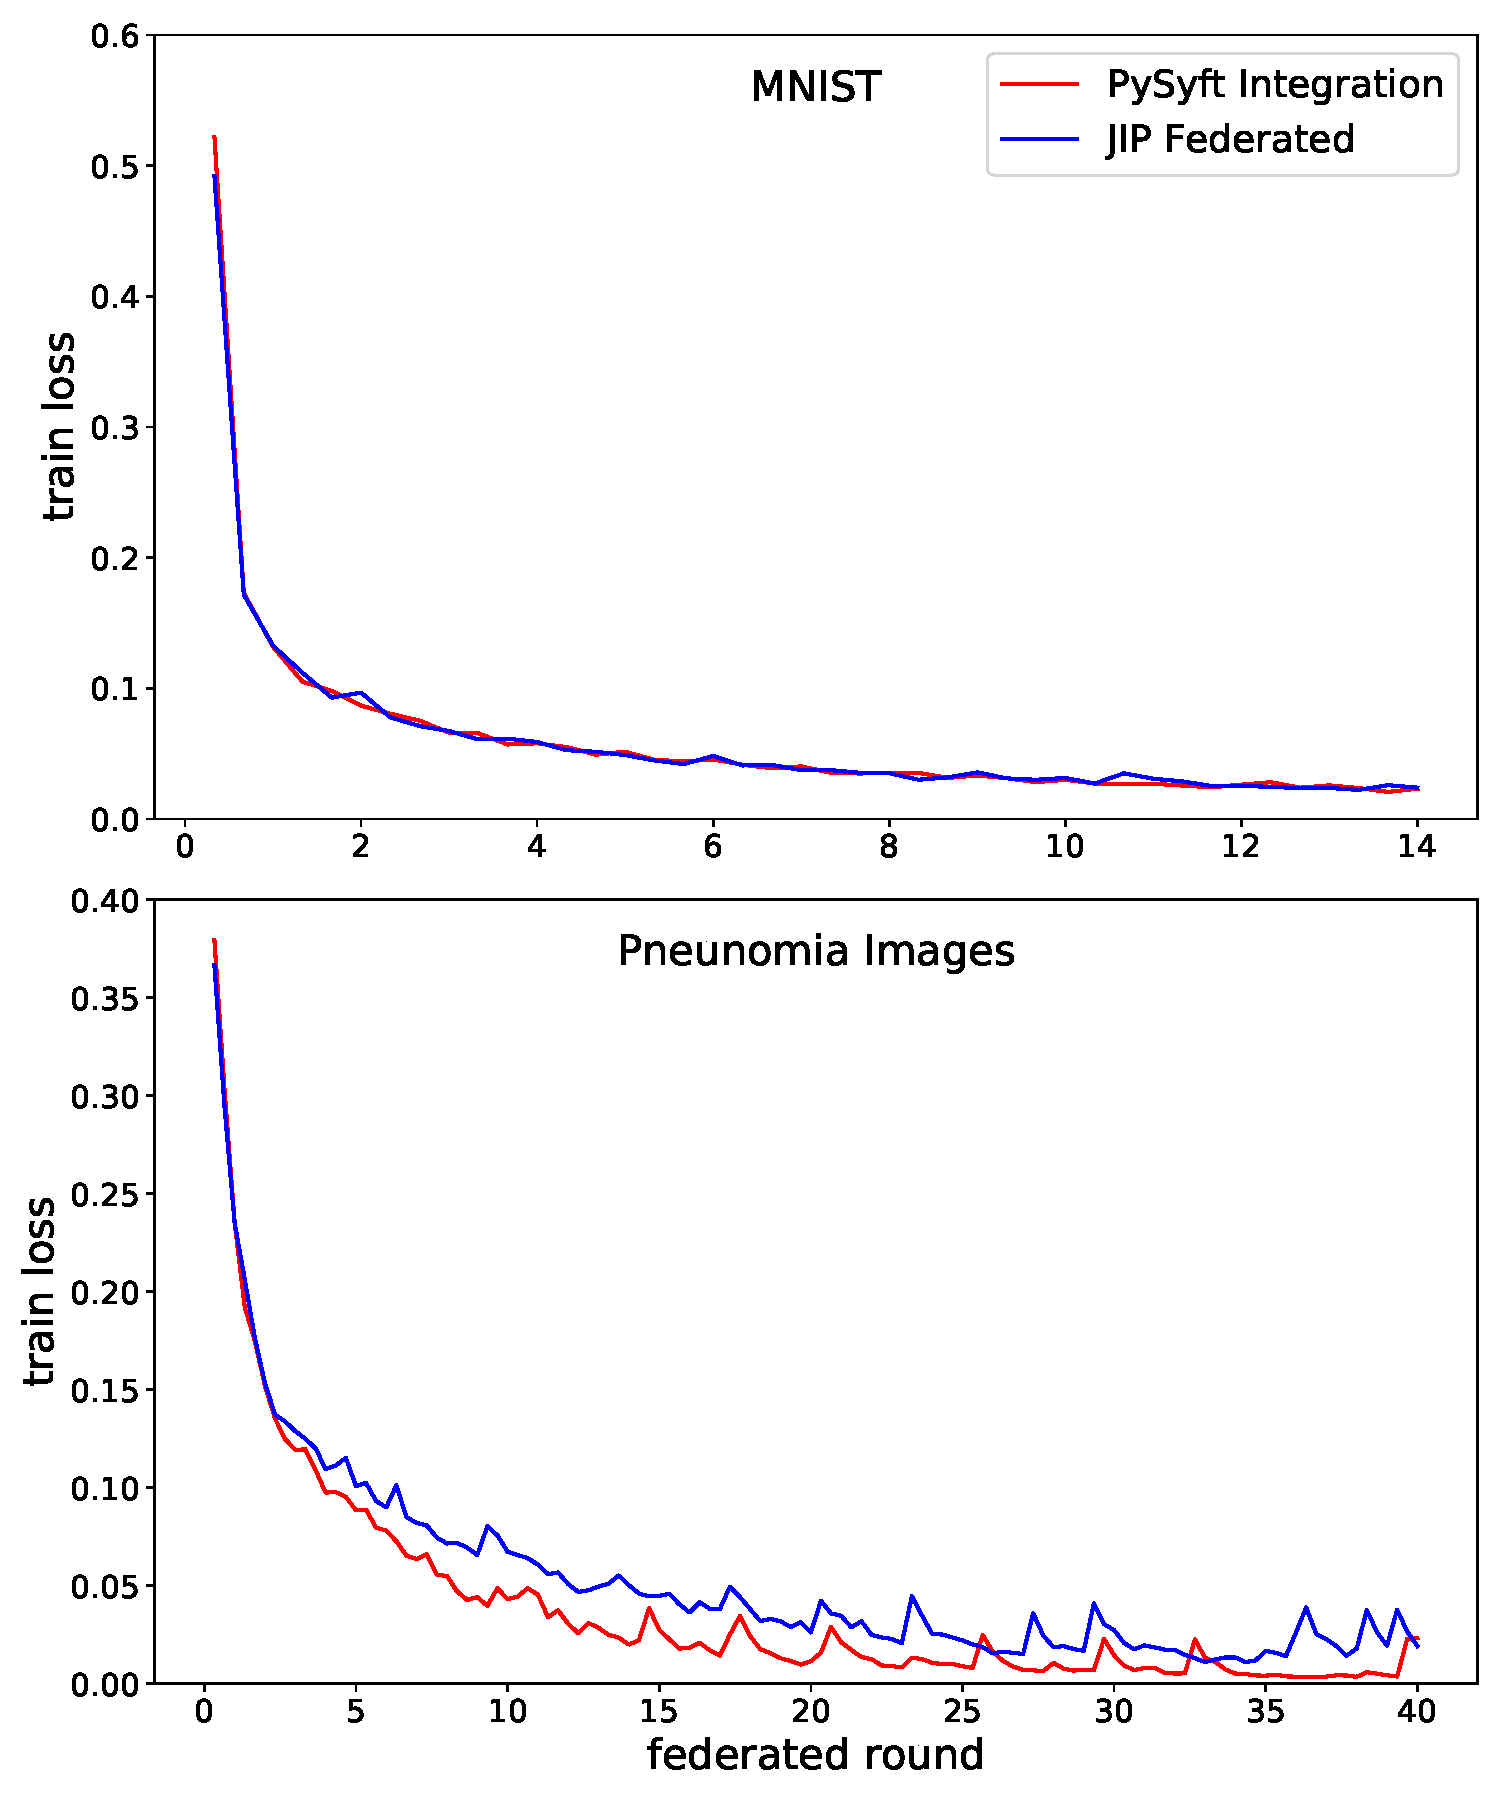
\includegraphics[width=1.0\textwidth]{1_Figures/RuntimeExperiments.pdf}}
    \centerline{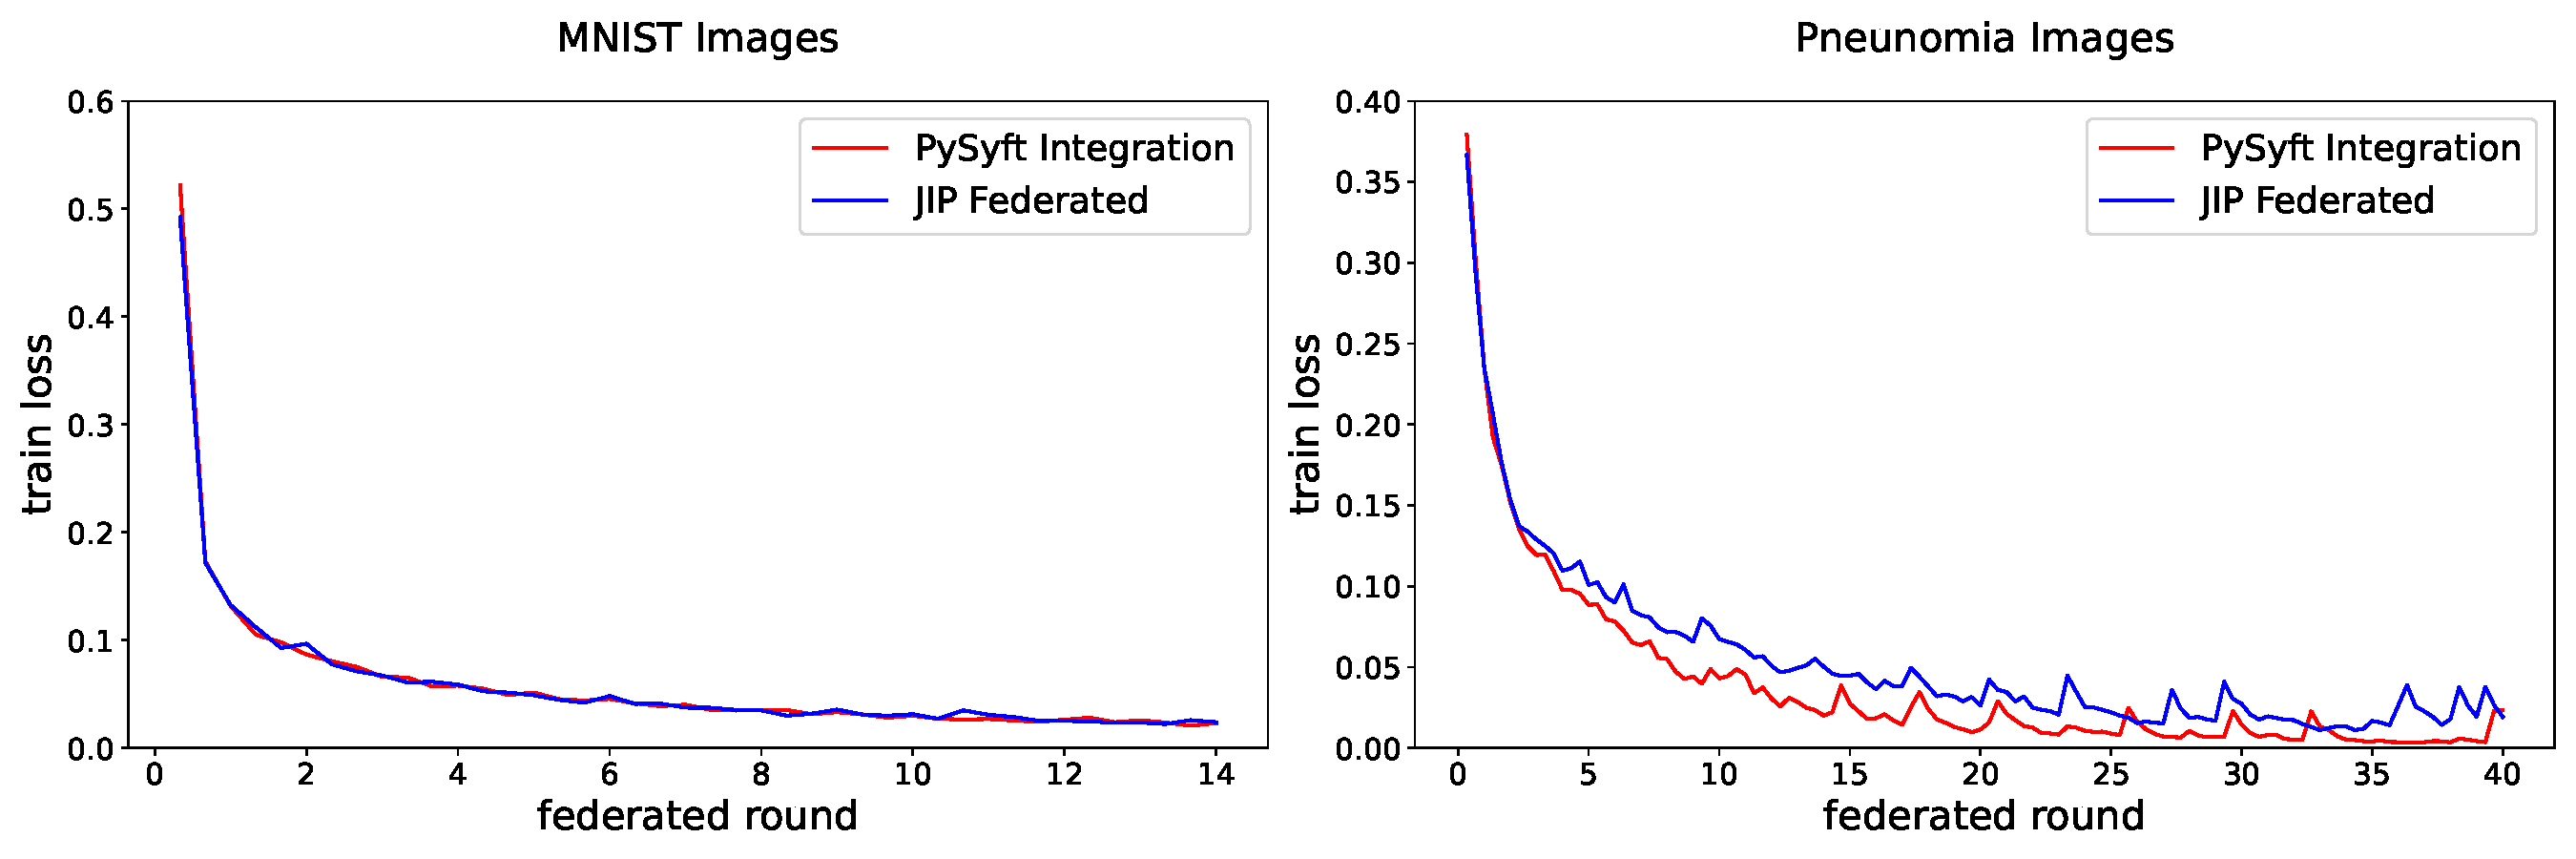
\includegraphics[width=1.0\textwidth]{1_Figures/RuntimeExperiments_horizontal.pdf}}
    \caption{Training loss on MNIST and the pneumonia dataset using the JIP's PySyft integration (red) and JIP Federated (blue).}
\label{fig:RuntimeExp}
\end{figure}

% Performance statistics
The performance of the final model checkpoints is compared using the accuracy on the held-out test data. 
For the experiments on the slightly unbalanced pneumonia dataset, the ROC-AUC is considered additionally. The scores are listed in \Cref{tab:Performance}.

\begin{table}[htbp]
  \centering
  \begin{tabular}{ccc}
  Experiment & Accuracy & ROC-AUC \\
  \hline \\[-2.5ex] %[-1.5ex]
  PySyft on MNIST               & 99.02 \% & - \\
  JIP Federated on MNIST        & 99.20 \% & - \\
  PySyft on pneumonia           & 91.35 \% & 0.887 \\
  JIP Federated on pneumonia    & 92.79 \% & 0.906 \\
 \end{tabular}
 \caption{Model performance on held out test data (one run).}
 \label{tab:Performance}
\end{table}
% PySyft MNIST:     99.02% 
% Kaapana MNIST:    99.20% 
% PySyft Chest:     91.346% (ROC-AUC: 0.887)
% Kaapana Chest:    92.788% (ROC-AUC: 0.906)

% Run time
\Cref{tab:RuntimeExp} lists the runtime differences between starting the first federated round and saving the final model of the conducted experiments.

%\begin{table}[h!]
\begin{table}[htbp]
  \centering
  \begin{tabular}{ccc}
  Implementation & MNIST & Pneumonia Images \\
  \hline \\[-2.5ex] %[-1.5ex]
  PySyft        & 01:46:32 & 20:51:21 \\
  JIP Federated & 01:38:50 & 08:55:03 \\
 \end{tabular}
 \caption{Runtime of conducted experiments (hh:mm:ss; one run)}
 \label{tab:RuntimeExp}
\end{table}






\subsection{JIP Federated Segmentation Experiment}
\label{subsec:ResultsSegmentation}

% Intro sentence
The segmentation experiment on the BraTS data serves to demonstrate that JIP Federated is capable of performing complex deep learning tasks. \textit{Federated Averaging} was used as an aggregation algorithm, and the model training was executed on GPU.

% TODO: Graph mit allen Plots drin!
\begin{figure}[htbp]
%\begin{figure*}[h!]
    %\centerline{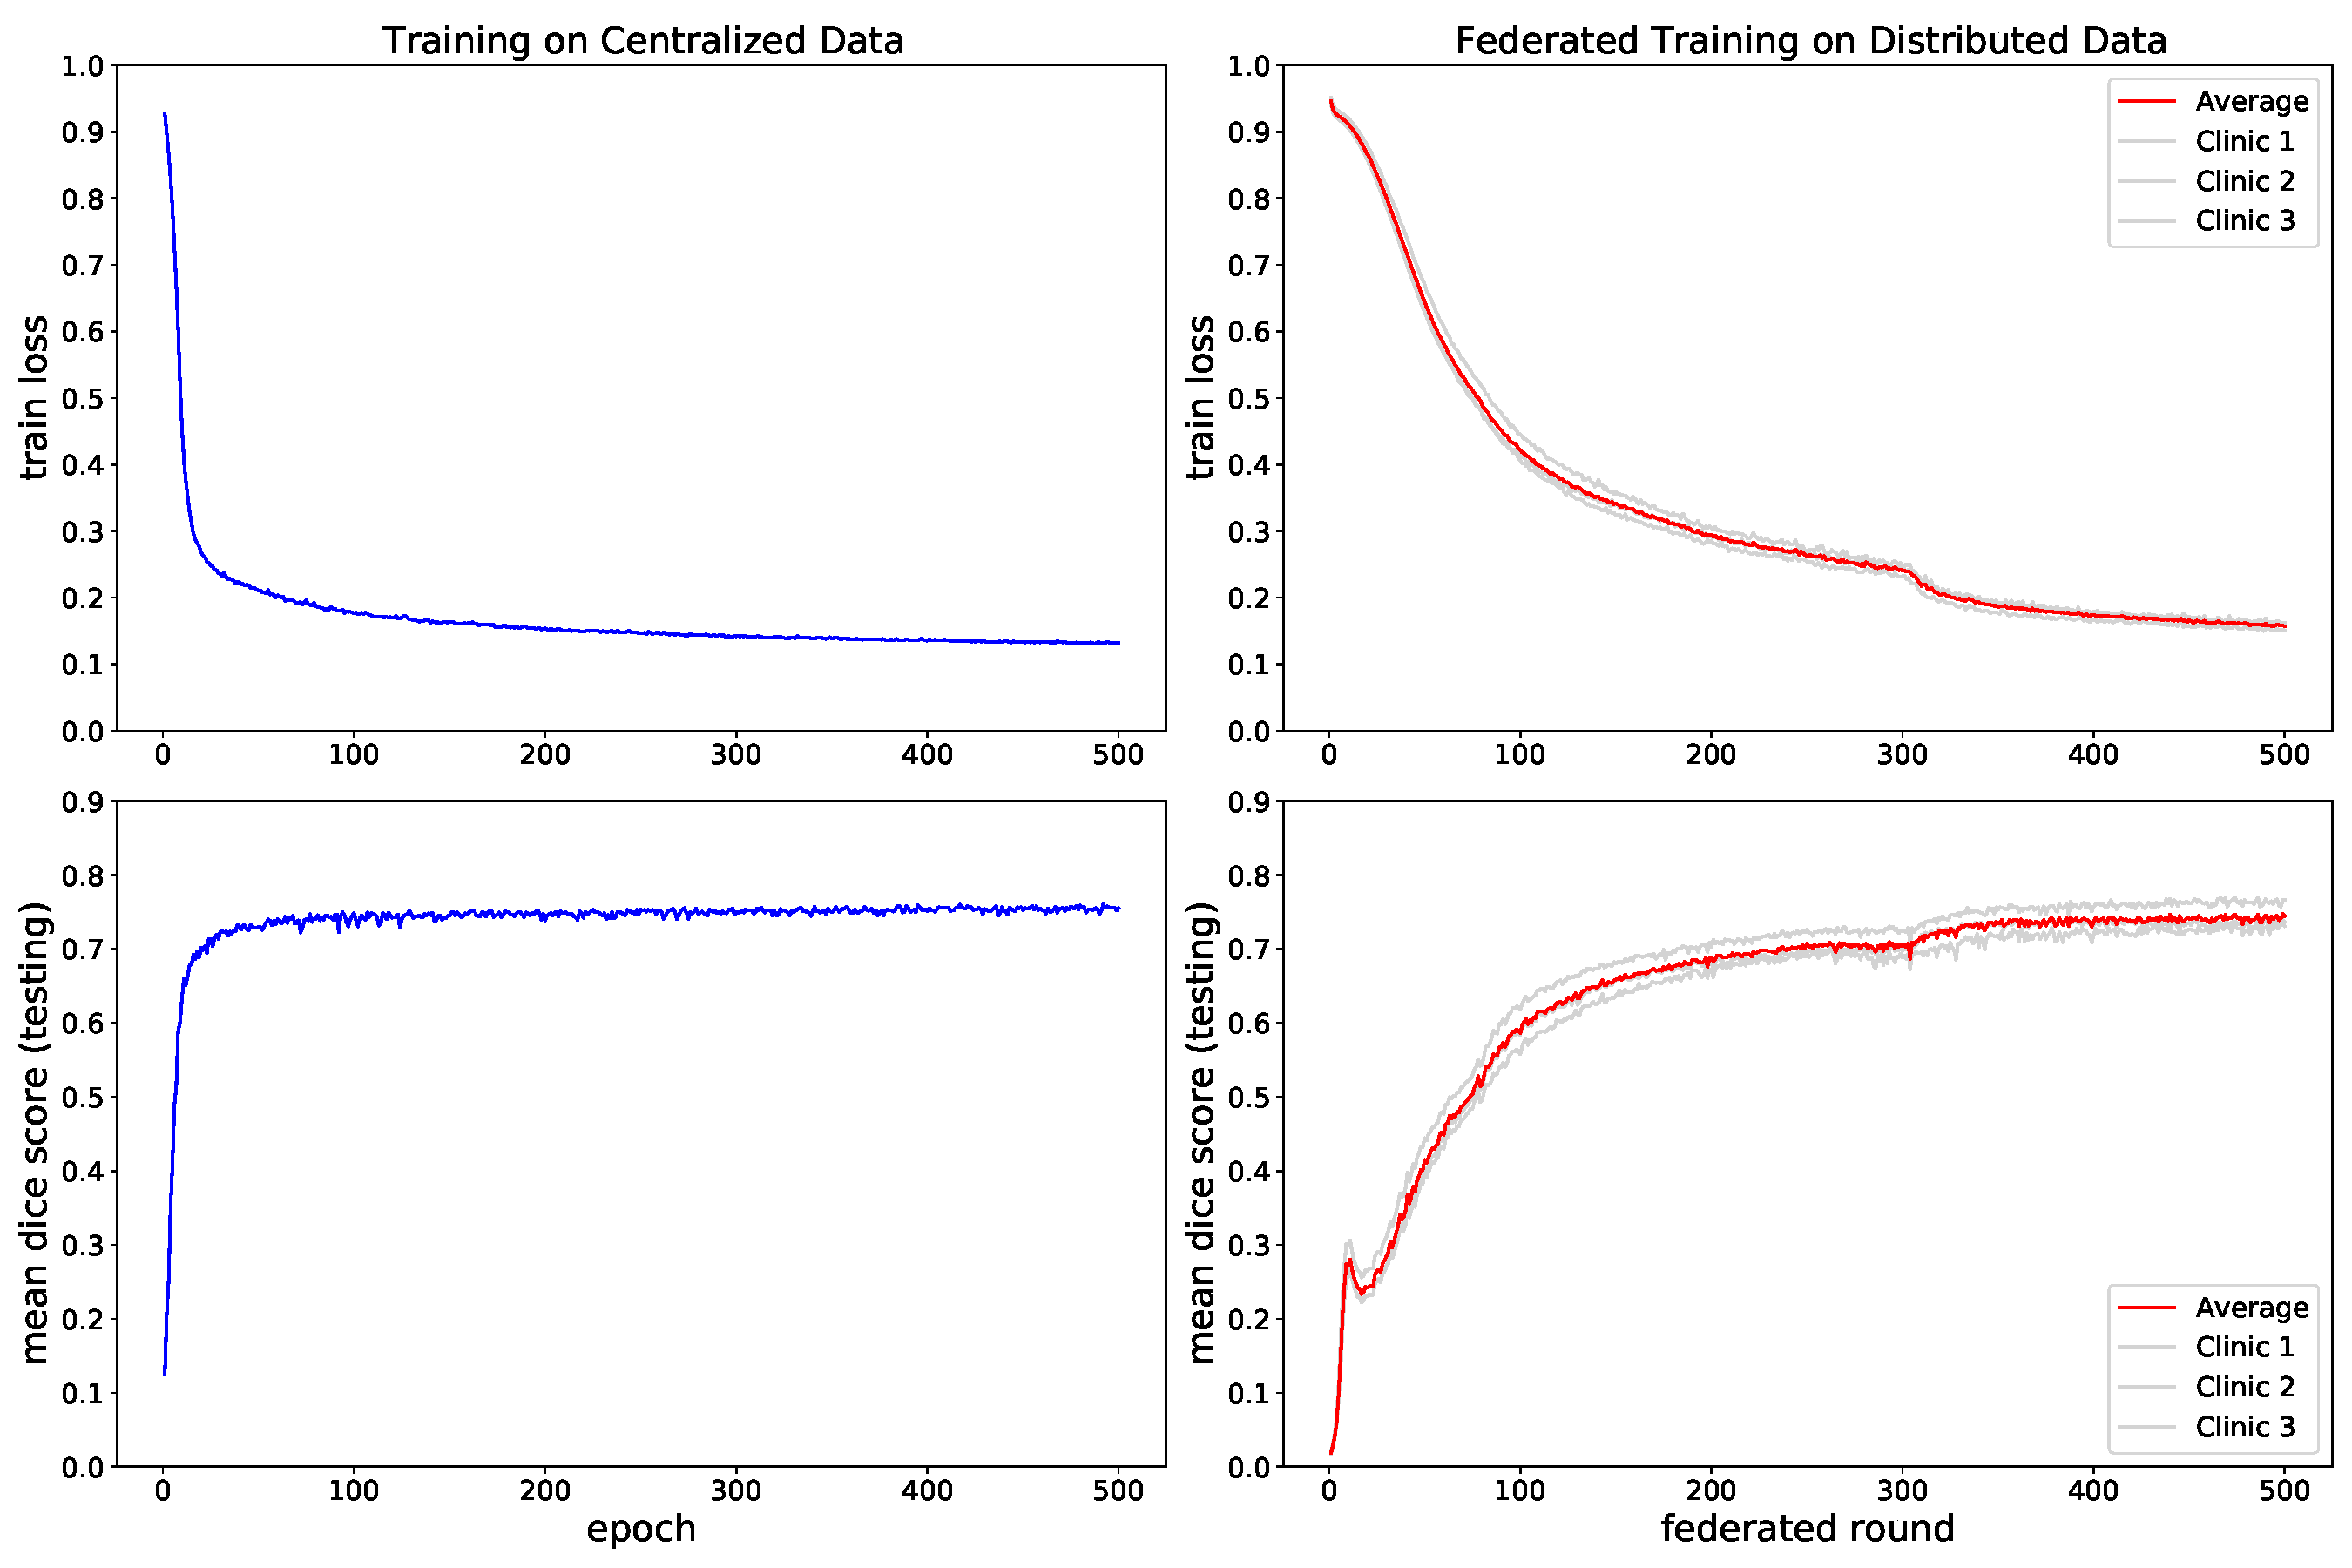
\includegraphics[width=1.0\textwidth]{1_Figures/BraTSexperiments.pdf}}
    \centerline{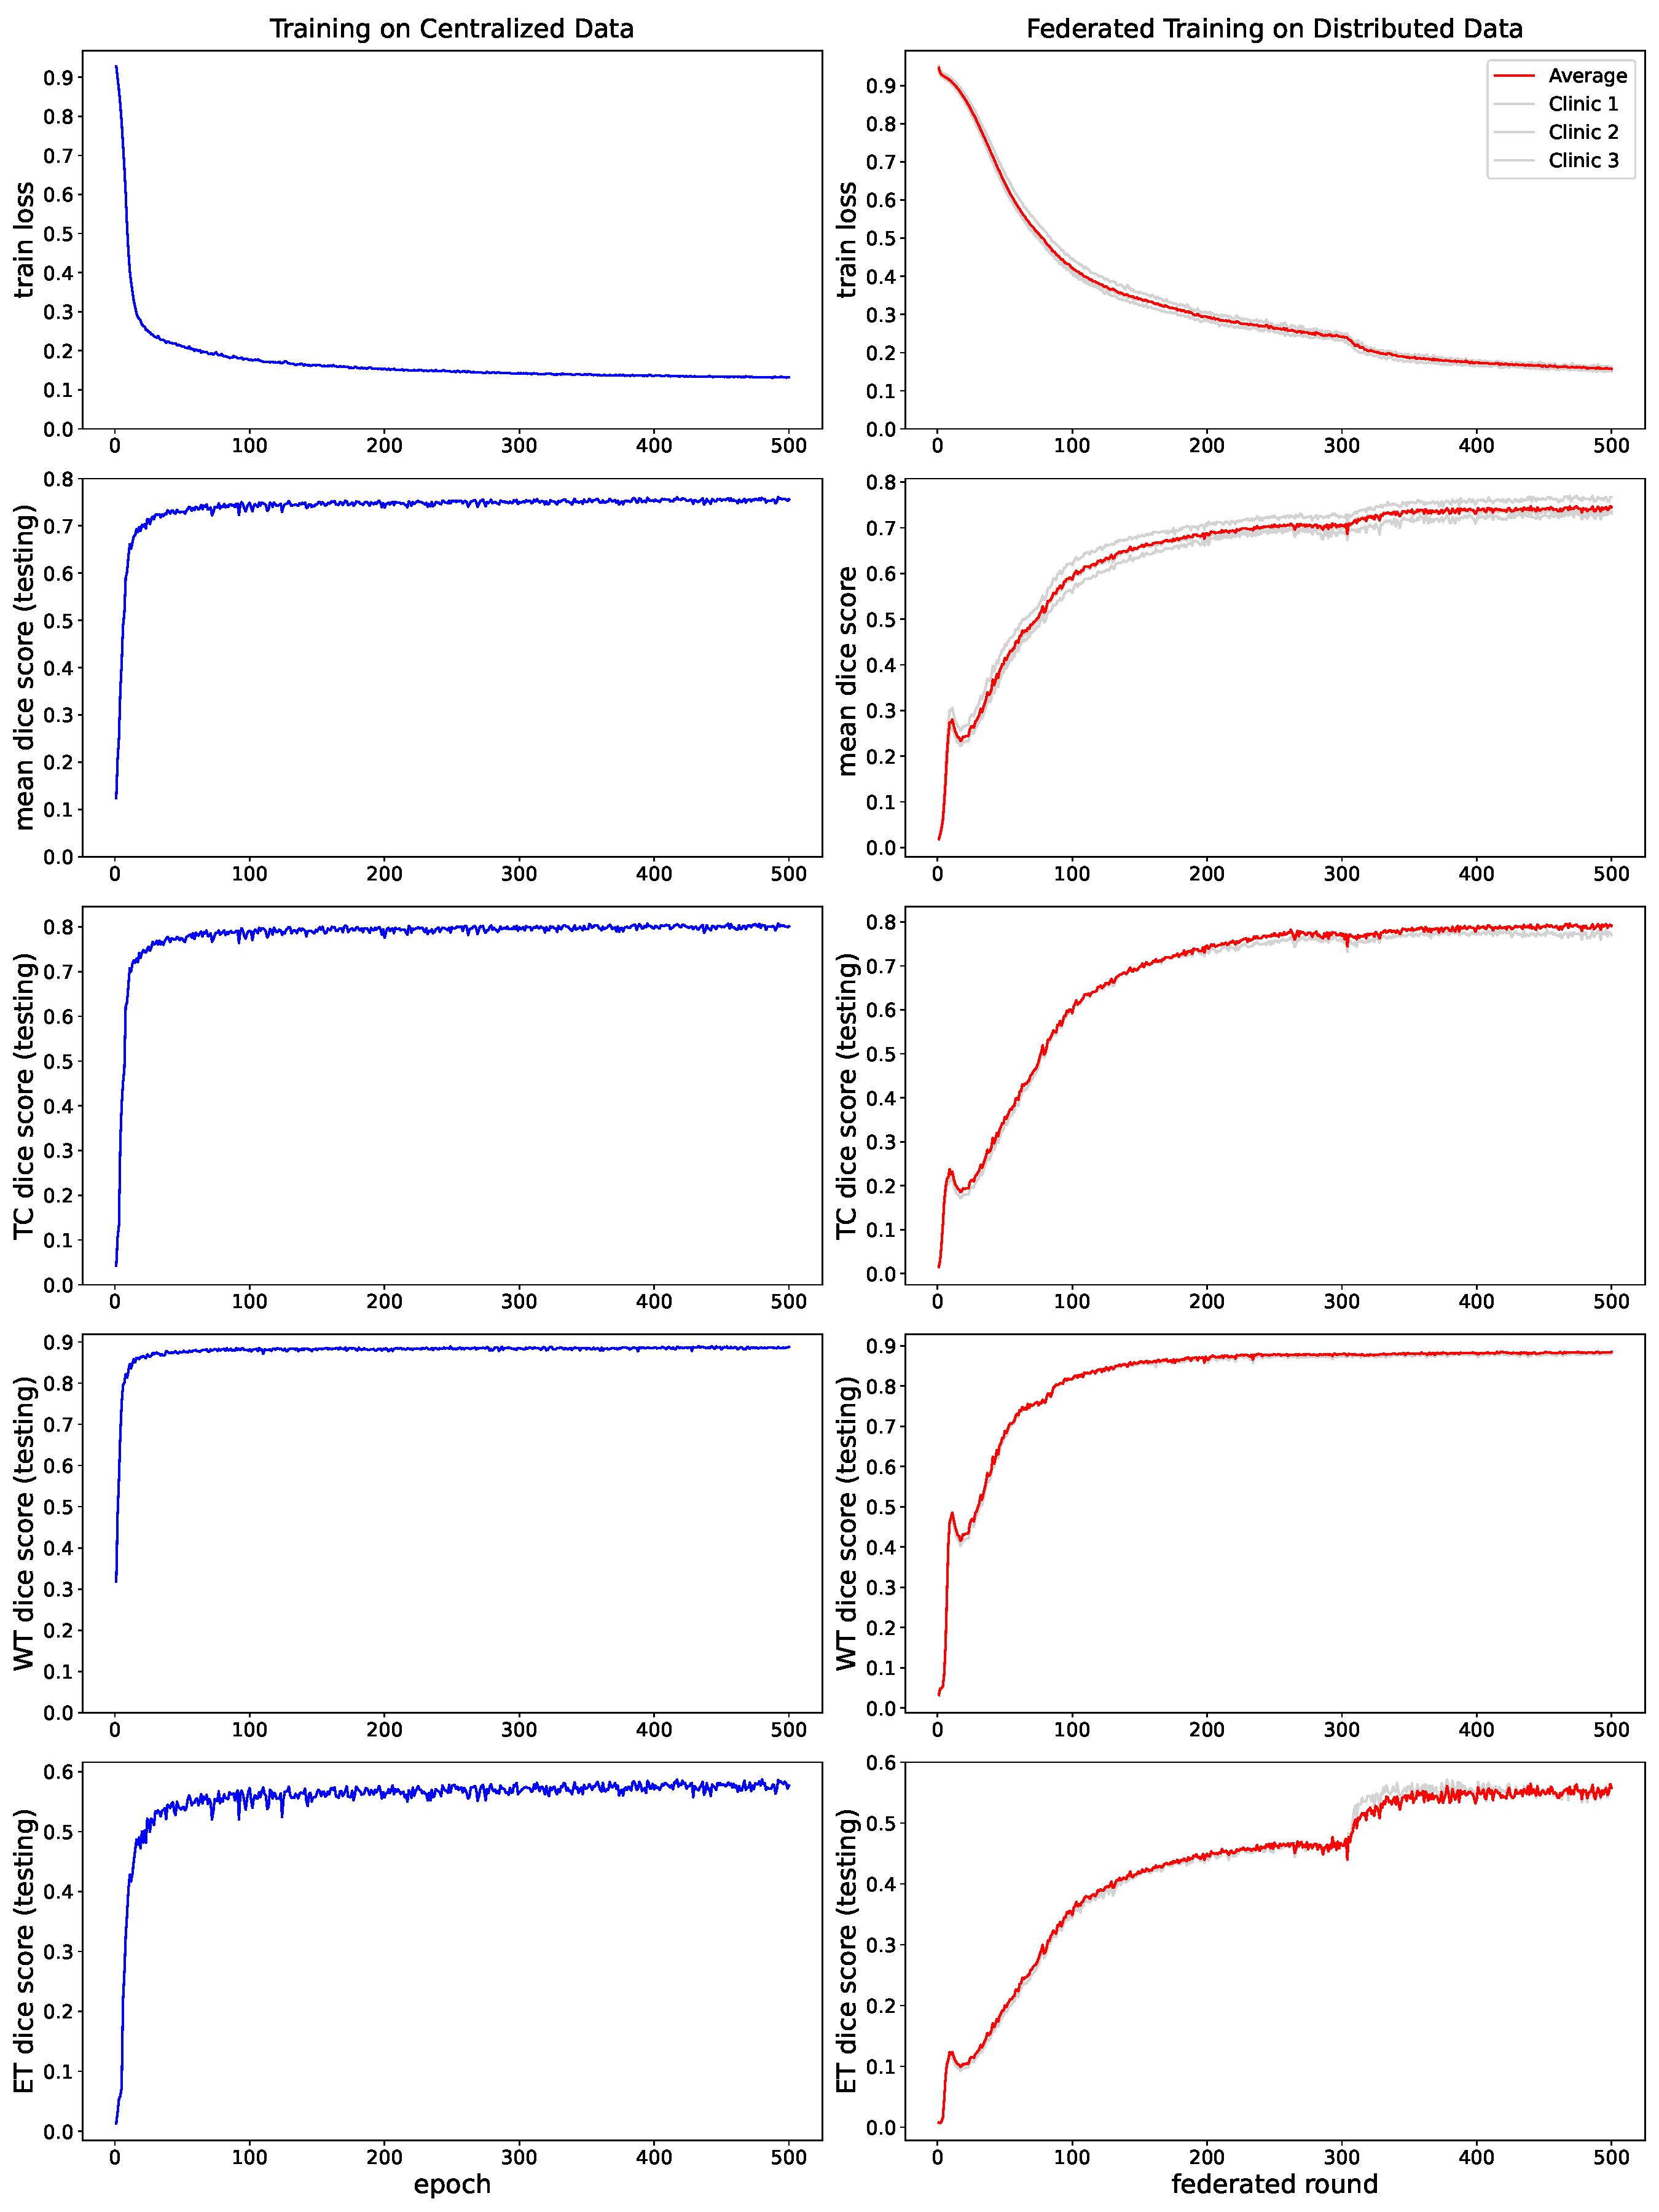
\includegraphics[width=1.0\textwidth]{1_Figures/BraTSexperiments_all.pdf}}
    \caption{Training loss and testing performance of models trained on centralized data (blue) and in a federated scenario across three participating clinics (red).}
\label{fig:BraTSplots}
\end{figure}


% mean dice score and figure
\Cref{fig:BraTSplots} shows the training loss together with the mean dice score on the test data for each federated round. The mean dice score is build as the average of the three given label masks (ET, TC, WT) described in \Cref{subsec:MethodsExperiments}. 
Each data point represents the mean value over one epoch, respectively, one iteration on the corresponding data.

% illustration
In order to imitate a realistic FL scenario, the test performance was computed locally on each participant using the test data available there. This results in three curves showing the local behavior. The local training loss and mean dice score of the participating clinics were aggregated to averaged values.
As upper baseline, the curves of the model training on the centralized data are also displayed.


% TODO: Anderern Plots erläutern